\subsection{Molecular Dynamics (MD)}
\label{section:tools:md}

Due to the high charge states seen in experiments with clusters the most
practical method to microscopically study the ionization dynamics is
\textit{Molecular Dynamics} (MD) where ions and electrons are treated
classically.

In MD, bodies interact directly through classical instantaneous forces. Even
though the method's name contains the term ``molecular'', these forces can be
of any nature; gravitational, van der Waals, Lennard-Jones, electrostatic, etc.
The method numerically integrates Newton's equations of motion, resulting in a
time evolution of the system.

The total force (from two-body interactions) acting on particle $i$ of mass
$m_i$ from all other $N$ particles in the system is:
\begin{align}
m_i \va_i & = \vF_i = \sum_{j \ne i} \vF_{j \rightarrow i}.
\label{eqn:md:newton}
\end{align}

In the present work, the force between charged particles is the instantaneous
electrostatic Coulomb force:
\begin{align}
\vF_{C,j \rightarrow i}\pa{\vr} & =\frac{k q_i q_j}{r_{ji}^2} \hvr_{ji}.
\label{eqn:md:coulomb:F}
\end{align}
which only depends on the distance $\vr_{ji}$ between particles and the charge
states $Z_i$ of these particles $q_i = Z_i e_0$ ($q_i$ is particle $i$'s charge
and $e_0$ is the elementary charge). In the case of electrons, the charge
state is simply -1.

Calculating $\vF_i$
from \eqref{eqn:md:newton} and \eqref{eqn:md:coulomb:F} requires one operation
per particle present in the system; updating the force on one particle is an
$O\pa{N}$ operation (doubling the number of particles will double the required
calculation time). Since there are $N$ particles, calculating the force for
all particles has a scaling of $O\pa{N^2}$ (doubling the number of
particles will quadruple the required calculation time). Some forces used in
different research areas are short range and can then be cut off at a certain
distance. This effectively reduces the scaling from $O\pa{N^2}$ to $O\pa{N}$
but the Coulomb potential, being long range, cannot be artificially cut off.
Chapter \ref{section:intro:md:tree} discusses a different algorithm that allows
a reduction to $O\pa{N \log{N}}$.


Figure
\ref{fig:md:vectors} shows the vector definitions used throughout this work. We
define particle $i$ as the particle we are interested in (for example, the
particle we are calculating the force on), and particle $j$ the particle that
is generating the field or potential that is measured at location of particle
$i$. We thus have:
\begin{align}
\vr_{j} + \vr_{j,i} & = \vr_{i}, \\
\vr_{j,i} & = \vr_{i} - \vr_{j}, \\
\hvr_{j,i} & = \frac{\vr_{j,i}}{\abs{\vr_{j,i}}}.
\end{align}
%       _j
%       /|\
%  r_j /   \ r_ji
%     /    _\/
%    /------>i
%       r_i
%
\begin{figure}
 \centering
 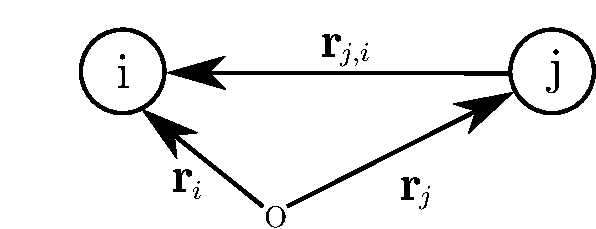
\includegraphics[width=0.5\columnwidth]{figures/vectors}
 \caption{\label{fig:md:vectors}Vectors definition between particles $i$ and $j$}
\end{figure}
%
%
Equation \eqref{eqn:md:newton} can be time integrated for every particle
$i$ using the Velocity-Verlet~(VV) scheme:
\begin{subequations}
\label{eqn:md:vv}
\begin{align}
\vx_{i}^{\pa{n+1}} & = \vx_{i}^{\pa{n}} + \vv_{i}^{\pa{n}} \Delta t +
\frac{\va_{i}^{\pa{n}}}{2} \Delta t^2, \\
\va_{i}^{\pa{n+1}} & = \frac{\vF^{\pa{n}}}{m_i}, \label{eqn:md:vv:a} \\
\vv_{i}^{\pa{n+1}} & = \vv_{i}^{\pa{n}} + \frac{\va_{i}^{\pa{n}} +
\va_{i}^{\pa{n+1}}}{2} \Delta t,
\end{align}
\end{subequations}
where $\Delta t$ is the integration time step, $\vx_{i}$ the position vector,
$\vv_{i}$ the velocity vector and $\va_{i}$ the acceleration vector, all evaluated
for particle $i$ at either the time step $n$ or the next one $n+1$.
Equations \eqref{eqn:md:vv}, when applied to every particle $i$ of the system,
can thus be used to propagate in time the whole cluster.

Every particle in the system stores its position $\vx^{\pa{n}}$, its velocity
$\vv^{\pa{n}}$ and also the total force acting on it $\vF^{\pa{n}}$. This total
force is the sum of all contribution of equation \eqref{eqn:md:coulomb:F} from
all other particles in the system.

The MD algorithm basically calculates the force between every pair of particles
in the system. Since there are $N$ total particles, there are $O\pa{N^2}$
interactions to calculate. Doubling the number of particles will quadruple the
computational burden, effectively putting an upper limit on the number of
particles that can be simulated to tens of thousands.

A cluster example can be seen on figure \ref{fig:md:cluster}.
This cluster is composed
of 147 xenon atoms (large blue spheres) and absorbs some photons (red
wave-packets) from the laser field. Atoms are ionized; electron are created
(small grey spheres) which move through the cluster. Ions are represented by
colours from blue for neutral to red for Xe$^{5+}$. The figure was
generated using
PyMOL\footnote{\textit{The PyMOL Molecular Graphics System}, Version 1.5.0.4,
Schrödinger, LLC. \url{http://pymol.org/}} on actual simulation-created data.


\begin{figure}
 % set opaque_background, off
 \centering
 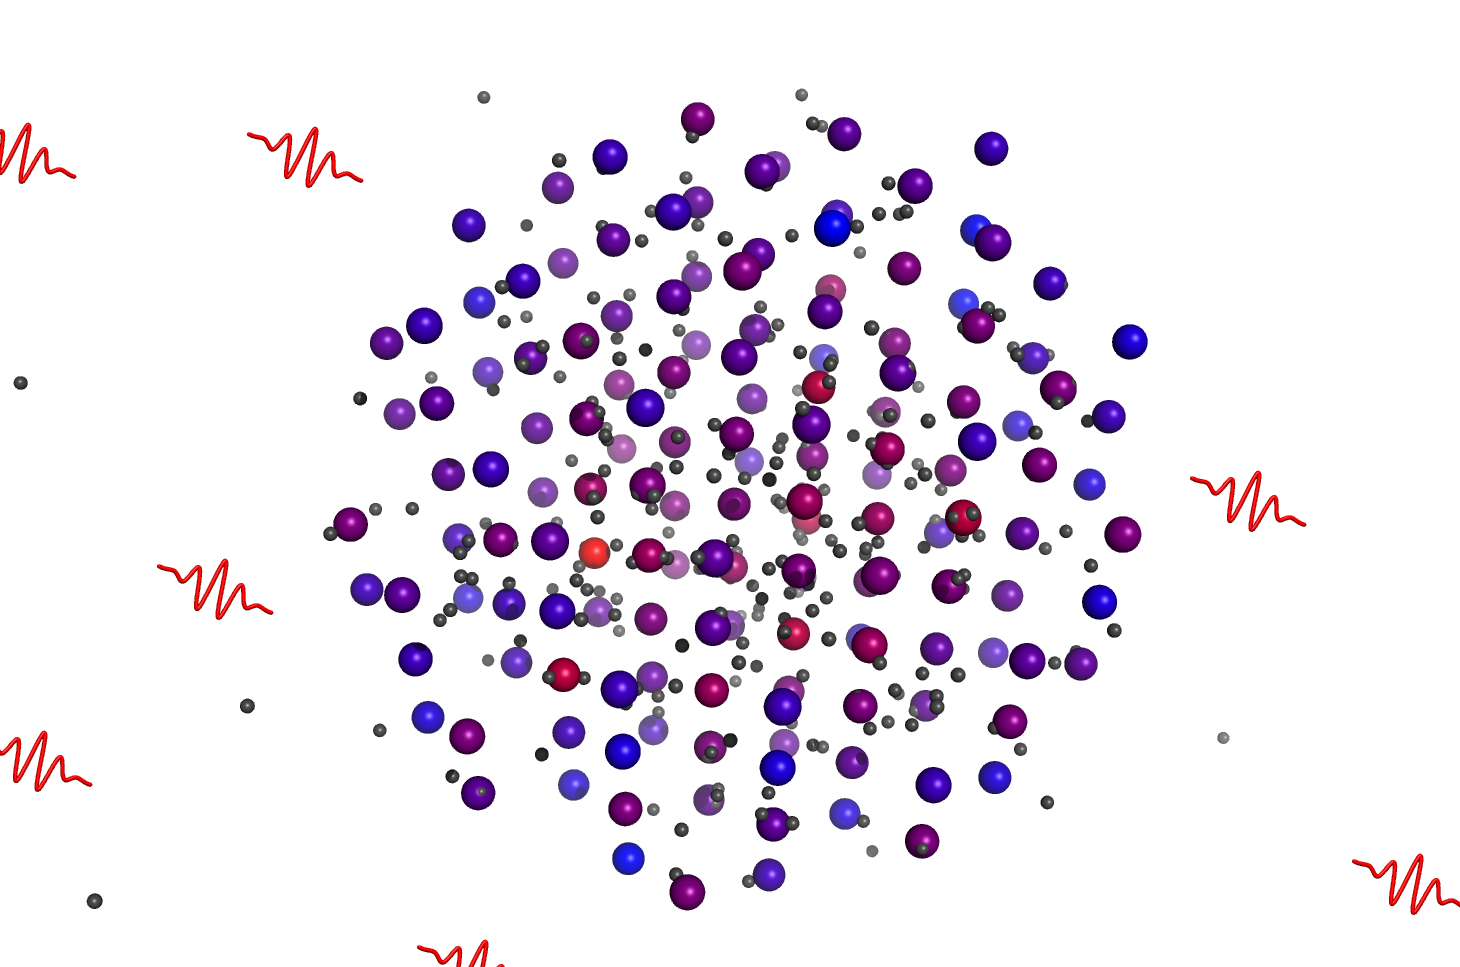
\includegraphics[width=\figurewidth]{figures/cluster}
 \caption{\label{fig:md:cluster}Example ionized Xe$_{147}$ cluster; xenon as
          large spheres with colours from blue for neutral to full red for
          Xe$^{5+}$, electrons in small grey spheres. Photons from the laser
          field are displayed as red wave-packets.}
\end{figure}

